\documentclass[hyperref]{ctexart}
\usepackage[left=2.50cm, right=2.50cm, top=2.50cm, bottom=2.50cm]{geometry} %页边距
\usepackage{helvet}
\usepackage{amsmath, amsfonts, amssymb} % 数学公式、符号
\usepackage[english]{babel}
\usepackage{graphicx}   % 图片
\usepackage{url}        % 超链接
\usepackage{bm}         % 加粗方程字体
\usepackage{multirow}
\usepackage{booktabs}
\usepackage{algorithm}
\usepackage{algorithmic}
\usepackage{fancyhdr} %设置页眉、页脚
\pagestyle{fancy}
\lhead{}
\chead{}
\lfoot{}
\cfoot{}
\rfoot{}
\usepackage{hyperref} %bookmarks
\hypersetup{colorlinks, bookmarks, unicode} %unicode
\usepackage{multicol}
\title{\textbf{放射性测量的统计误差}}
\author{\sffamily 赵宇航}
\date{}
\begin{document}
\maketitle
\indent{\bf 摘要: }本实验利用虚拟设备测量了放射源在固定时间的粒子数,分别以泊松分布和高斯分布拟合,计算其统计误差,分析了精度,验证了原子核衰变及放射性计数的统计规律。\\	
\begin{multicols}{2}
\CTEXsetup[format={\Large\bfseries}]{section}
\section{实验目的}
1.验证原子核衰变及放射性计数的统计规律。

2.了解统计误差的意义,掌握计算统计误差的方法。

3.掌握对测量精度的要求,合理选择测量时间的方法。
\section{实验原理}
放射性原子核的衰变是彼此独立的。我们无法预知每个原子核的衰变时刻,也不能知道两次原子核衰变的时间的间隔。所以在重复的放射性测量中,即使保持完全相同的实验条件,每次测量的结果也不完全相同,而是围绕着其平均值上下涨落。也有可能差别很大。

这种现象就叫做放射性计数的统计性。放射性计数的这种统计性反映了放射性原子核衰变本身的固有特性,与使用的测量仪器及技术无关。放射性测量就是在衰变的统计涨落影响下进行的,因此了解统计误差的规律,对评估测结果的可靠性是很必要的。
\subsection{核衰变的统计规律}
放射性原子核的衰变可以看成是伯努里试验问题。设在$t=0$时,放射性原子核的总数是$N_0$,在$t$时间内将有一部分核发生了衰变。已知任何一个核在$t$时间内衰变的概率为$W=1-e^{-\lambda t}$,不衰变的概率为$q=1-W=e^{-\lambda t}$,$\lambda$是该放射性原子核的衰变常数。利用二项式分布可以得到总核数$N_0$在$t$时间内有$N$个核发生衰变的概率 $W(N)$为
\begin{equation}W(N)=\frac{N_0!}{(N_0-N)!N!}(1-e^{-\lambda t})^N(e^{-\lambda t})^{N_0-N}\end{equation}

在$t$时间内,衰变掉的原子核平均数为\begin{equation}\overline{N}=N_0W=N_0(1-e^{-\lambda t})\end{equation}
其相应的均方差为\begin{equation}\sigma=\sqrt{N_0Wq}=(\overline{N}e^{-\lambda t})^{\frac{1}{2}}\end{equation}
假如$\lambda t<<1$,即时间$t$远比半衰期小,这时$\sigma$可简化为\begin{equation}\sigma=\sqrt{\overline{N}}\end{equation}

$N_0$总是一个很大的数目,而且如果满足$\lambda t<<1$,则二项式分布可以简化为泊松分布。在二项式分布中,$N_0$不小于$100$,而且$W$不大于$0.01$的情况下,泊松分布能很好的近似于二项式分布。此时几率分布可写成\begin{equation}W(N)=\frac{\overline{N}^N}{N!}e^{-\overline{N}} \label{bs}\end{equation}
当$N\geq 20$时,泊松分布一般就可用正态(高斯)分布来代替。\begin{equation}W(N)=\frac{1}{\sqrt{2\pi \sigma}}e^{\frac{-(N-\overline{N})^2}{2 \sigma^2}}\end{equation}式中$\sigma^2=\overline{N}$,$W(N)$是在 N 处的概率密度值。

我们在实际测量中,当测量时间$t$小于放射性核的半衰期时,可以用一次测量结果$N$来代替平均值,其统计差为$\sigma=\sqrt{N}$,测量结果可以写成\begin{equation}N\pm\sqrt{N}\label{wucha}\end{equation}

它的物理意义表示在完全相同的条件下再进行一次测量,其测量值处于$N-\sqrt{N}$到$N+\sqrt{N}$范围内的几率为$68.3\%$,用数理统计的术语来说,我们把$68.3\%$为“置信度”。相应的置信区间为$N\pm\sigma$,而当置信区间为$N\pm 2\sigma$和$N\pm3\sigma$时,相应的置信度为$95.5\%$和$99.7\%$,测量的相对误差为\begin{equation}\delta=\frac{\sigma}{N}=\frac{\sqrt{N}}{N}=\frac{1}{\sqrt{N}}\label{delta}\end{equation}
$\delta$可以用来说明测量的精度,当$N$大时$\delta$小,表示测量精度高;当$N$小时$\delta$大,表示测量精度低。
\subsection{测量时间的选择}
测量放射性时,一般对计数率$n=\frac{N}{t}$(脉冲数/秒)或放射性的衰变率$A$(衰变数/秒)感兴趣,因为时间$t$的测量不受统计涨落影响,所以\begin{equation}\frac{N\pm\sqrt{N}}{t}=\frac{N}{t}\pm\frac{\sqrt{N}}{t}\end{equation}
因此计数率的统计误差可表示为\begin{equation}n\pm\sqrt{\frac{n}{t}}=n(1\pm\frac{1}{\sqrt{N}})\label{tjwc}\end{equation}

只要计数$N$相同,计数率和计数的相对误差是一样的。当计数率不变时,测时间越长,误差越小;当测量时间被限定时,则计数率越高,误差越小。

如果进行$m$次重复测量,总计数为$N_0$,平均计数为$\overline{N}$,总计数和误差用$m\overline{N}\pm\sqrt{m\overline{N}}$表示,平均计数及统计误差可表示为\begin{equation}N\pm\sqrt{\frac{\overline{N}}{m}}=n(1\pm\frac{1}{\sqrt{N_0}})\label{jswc}\end{equation}
由此可见,测量次数越多,误差越小,精确度越高。但$m$次测量总计数$N$,和平均值$\overline{N}$的相对误差是一样的。

在测量较强的放射性时,必须对测量结果进行由于探测系统分辨时间不够小所引起的漏计数的校正。而在低水平测量中,必须考虑到本底计数的统计涨落。所谓本底涨落是由于宇宙线和测量装置周围有微量放射性物质的沾染等原因造成的。本底计数也服从统计规律。考虑本底的统计误差后,源的净计数率的数学表达式为\begin{equation}n\pm\sigma_n=(n_s-n_b)\pm\sqrt{\frac{n_s}{t_s}+\frac{n_b}{t_b}}\end{equation}
而相对误差为\begin{equation}\delta=\sqrt{\frac{n_s}{t_s}+\frac{n_b}{t_b}}/(n_s-n_b)\end{equation}式中$n_s$为测量源加本底的总计数率,$n_b$为没有放射源时的本底计数率,$t_s$为有源时的测量时间,$t_b$为本底测量时间。

从上式可以看出:

1.本底计数率越大,对测量精度的影响越大,因此在测量时应很好屏蔽,想方设法或减小本底计数率。

2.为了减少$n$的误差应增加$t_s$和$t_b$,但过长的测量时间对我们并不利,故要选择合适的测量时间。一般是在限定的误差范围内,确定最短的测量时间;或者是在总测量时间一定时合理地分配$t_s$和$t_b$,以获得最小的测量误差。根据$\frac{d\sigma_n}{dt_s}=0$或$\frac{d\sigma_n}{dt_b}=0$可以求出,当$\frac{t_s}{t_b}=\sqrt{\frac{n_s}{n_b}}$时统计误差具有最小值。被测样品放射性愈强,本底测量时间就愈短,究竟选用多长的测量时间,由测量精度决定。由\eqref{delta}、\eqref{tjwc}式可以导出在给定的计数率相对误差$\delta$的情况下,样品的本底测量时间各为\begin{equation}\begin{split}t_s=\frac{n_s+\sqrt{n_s n_b}}{(n_s-n_b)^2\delta^2} \\ t_b=\frac{n_b+\sqrt{n_s n_b}}{(n_s-n_b)^2\delta^2}\end{split} \label{tstb}\end{equation}
\section{实验结果}
\subsection{泊松分布}
在模拟泊松分布中,我们以$0.2$秒计一次粒子数,共计数$4946$次。所得实验结果如下表所示。

\begin{center} 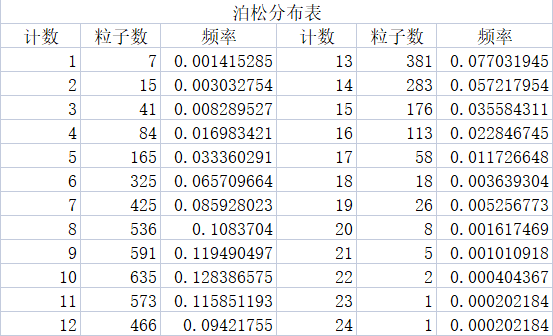
\includegraphics[scale=0.4]{bsbg.png} \label{bsbg} \end{center}

根据实验结果,我们作出泊松分布的频率直方图。

\begin{center}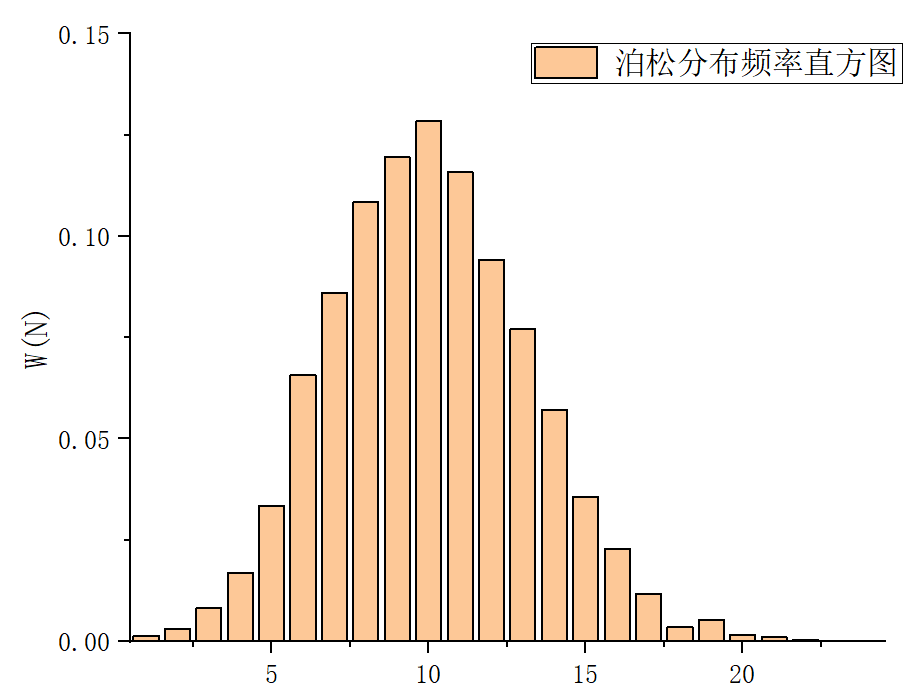
\includegraphics[scale=0.2]{bsfb.png} \end{center}

我们计算出$\overline{N}\approx 10.03255$,由式\eqref{bs} 绘出理论曲线,并和实验点线图比较,如下图所示。

\begin{center}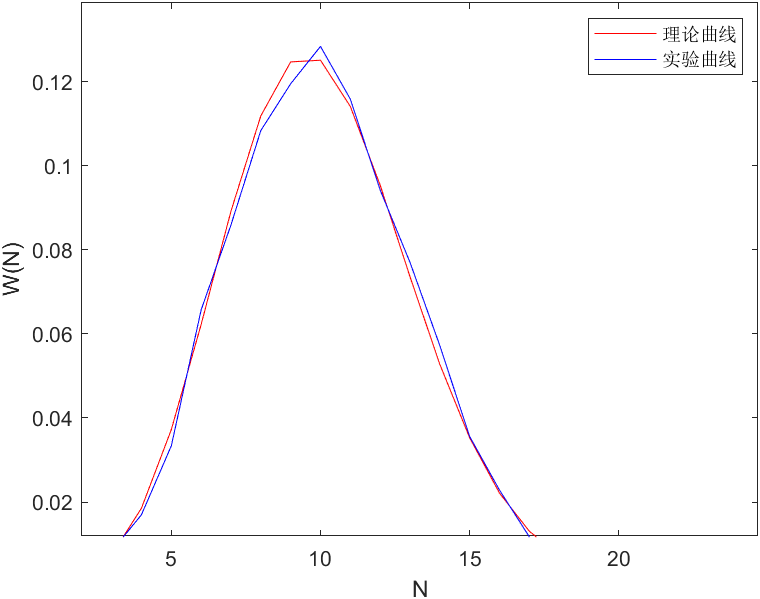
\includegraphics[scale=0.5]{bsqx.png} \end{center}

利用公式\begin{equation}\sigma_{\overline{N}}=\sqrt {\frac {\Sigma (N_i-\overline{N})^2}{n(n-1)}}\label{jfc}\end{equation}可以求出$\overline{N}$的误差是$2.54$。利用式\eqref{wucha},用$\overline{N}$近似一次测量可以求得一次测量的误差是$3.17$。
$\overline{N}\pm \sigma$即区间$(6.86,13.2)$,利用频率直方图可求得频率为$0.729$;$\overline{N}\pm 2\sigma$即区间$(3.69,16.37)$,利用频率直方图可求得频率为$0.961$;$\overline{N}\pm 3\sigma$即区间$(0.52,19.54)$,利用频率直方图可求得频率为$0.994$。

以$24$种粒子检验是否满足卡方分布,取显著性水平$\alpha=0.05$,查表知$\chi^2_{\alpha}(23)\approx 35.17$。利用公式\begin{equation}\chi^2=\sum^k_{i=1} \frac{n}{p_i}(\frac{f_i}{N}-p_i)^2 \label{gll}\end{equation}可以算得$\chi^2 \approx 13.93 \le 35.17$,所以可以接受假设。
\subsection{高斯分布}
在模拟高斯分布中,我们以$1$秒计一次粒子数,共计数$1004$次。所得实验结果如下表所示。

\begin{center} 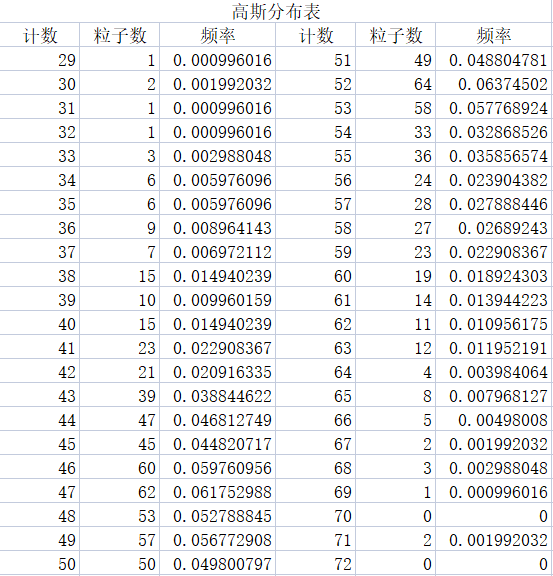
\includegraphics[scale=0.4]{gsbg.png} \label{gsbg} \end{center}

根据实验结果,我们作出泊松分布的频率直方图。

\begin{center}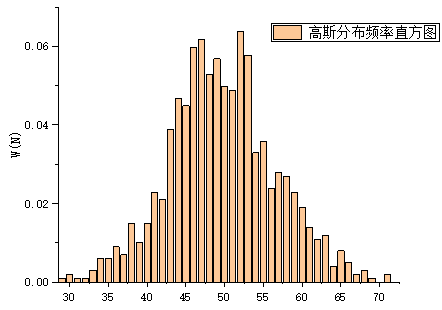
\includegraphics[scale=0.4]{gsfb.png} \end{center}

我们计算出$\overline{N}\approx 49.69323$,由式\eqref{bs} 绘出理论曲线,并和实验点线图比较,如下图所示。

\begin{center}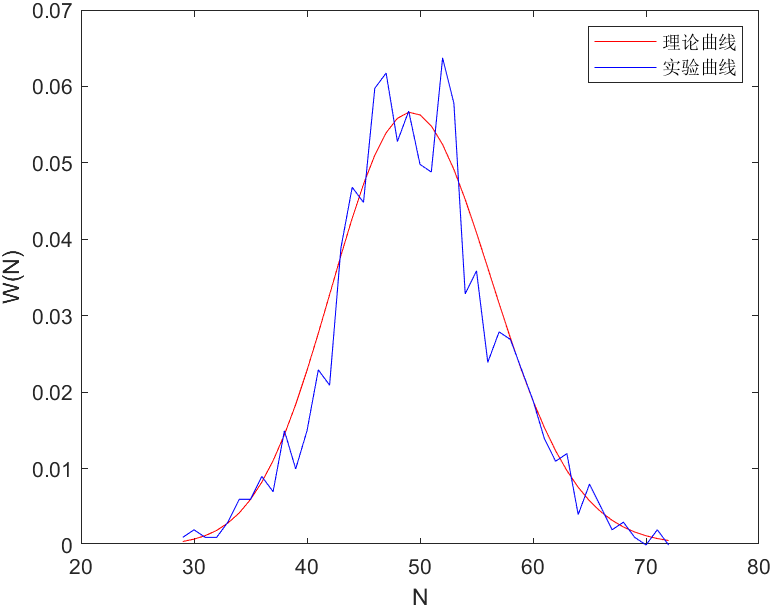
\includegraphics[scale=0.5]{gsqx.png} \end{center}

利用公式\eqref{jfc}可以求出$\overline{N}$的误差是$5.18$。利用式\eqref{wucha},用$\overline{N}$近似一次测量可以求得一次测量的误差是$7.05$。
$\overline{N}\pm \sigma$即区间$(42.64,56.74)$,利用频率直方图可求得频率为$0.674$;$\overline{N}\pm 2\sigma$即区间$(35.59,63.79)$,利用频率直方图可求得频率为$0.907$;$\overline{N}\pm 3\sigma$即区间$(28.54,70.84)$,利用频率直方图可求得频率为$0.998$。

以$41$种粒子检验是否满足卡方分布,取显著性水平$\alpha=0.05$,查表知$\chi^2_{\alpha}(23)\approx 55.76$。利用公式\eqref{gll}可以算得$\chi^2 \approx 38.94 \le 55.76$,所以可以接受假设。
\section{讨论}
放射性原子核衰变的统计性指由于放射性原子核的衰变是彼此独立,我们无法预知每个原子核的衰变时刻,也不能知道两次原子核衰变的时间的间隔。所以在重复的放射性测量中,即使保持完全相同的实验条件,每次测量的结果也不完全相同,而是围绕着其平均值上下涨落。
在实验中,$N_0$比较大而$W$比较小时,用泊松分布;单个的$N$比较大时,可以近似地用高斯分布。具体来说,当在二项式分布中,$N_0$不小于$100$,而且$W$不大于$0.01$的情况下,泊松分布能很好的近似于二项式分布。当$N\geq 20$时,泊松分布一般就可用正态(高斯)分布来代替。

$\sigma$指一次测量的统计差,利用式\eqref{wucha}可以以单次测量值$N$如何表示放射性测量值。它的物理意义表示在完全相同的条件下再进行一次测量,其测量值处于$N-\sqrt{N}$到$N+\sqrt{N}$范围内的几率为$68.3\%$。

注意到当$\frac{t_s}{t_b}=\sqrt{\frac{n_s}{n_b}}$时统计误差具有最小值,联立式\eqref{tstb}可以求得$t_s=150+50\sqrt{3}$
,$t_b=50+50\sqrt{3}$。

$^{137}Cs$的$\gamma$射线计数的统计误差可由式\eqref{jswc}得到,计数率的统计误差可由式\eqref{tjwc}得到。
\end{multicols}
\end{document}